\subsection{Low Energy \piz Production}\label{sec:into:xsection.low}

\begin{figure}[h!]\begin{center}
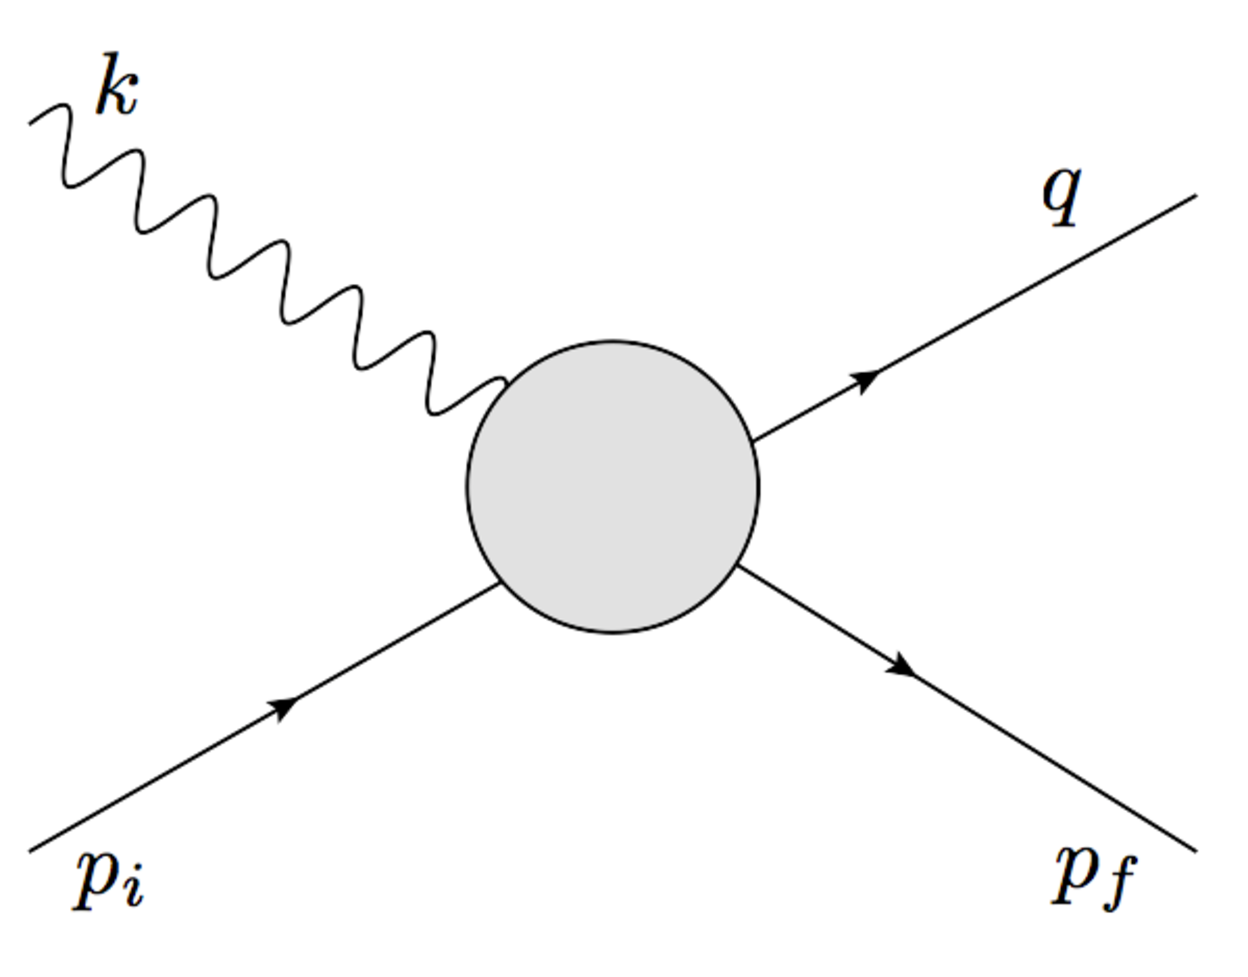
\includegraphics[width=0.5 \figwidth,height= \qfigheight]{\figures/feyman_pi0IV.pdf}
\caption[Diagram for photoproduction of the \piz meson]{\label{fig:xsection.pi0feynman}	Diagram for photoproduction of the \piz meson. $k$ and $p_i$ are the incident photon beam and target proton 4-moment respectively, $q$ and $p_f$ represent the produced \piz meson and scattered proton 4-momenta respectively.}
\end{center}\end{figure}
For incoming photon beam energies less than 2.8~GeV, the production of the \piz meson, with 4-momenta $q$, in photon-proton reactions, with 4-momenta $k$ and $p_i$ respectively and $p_f$ being the 4-momenta of the scattered proton (see Fig.~\ref{fig:xsection.pi0feynman}),  can be described in terms of the three Lorentz invariant Mandelstam variables, $s$, $t$ and $u$, where
\begin{align}
s = (k+p_i)^2 = (q+p_f)^2 \nonumber \\
t=(p_i-p_f)^2 = (k-q)^2  \nonumber \\
u = (k - p_f)^2 = (p_i-q)^2 \ .
\end{align}
The sum of the Mandelstam variables linearly combine to give the sum of masses of the particles involved:
\begin{align}
s + t + u = \sum\limits_{i}^{4} m_i^2 
\end{align}
and the definition of Lorentz-invariant mass:
\begin{align}
p_i\cdot p_i = E_i^2 - \mathbf{p_i}\cdot \mathbf{p_i} = m_i^2 \ .
\end{align}
Using energy-momentum conservation:
\begin{align}
k + p_i = q+p_f \,
\end{align}
it is seen that only three of the four momenta are independent. Conventionally the use of $k$ and $q$ and a combined 4-momenta of the nuclei 
\begin{align}
P = \frac{1}{2}(p_i+p_f)
\end{align}
are used as the independent kinematic variables. The three Mandelstam variables can be express in terms of the other two, therefore the scattering process is described by functions of only two of the Mandelstam variables. Conventionally they are chosen to be $s$ and $t$, which in the center-of-mass frame (C.M.) of the initial and final state equal the invariant mass squared of the system and the momentum transfer in the production process respectively.
\subsection{Isospin Representation}\label{sec:isospin}
The scattering matrix $\mathcal{M}$ for single pion photoproduction process is written as:
\begin{align}
\mathcal{M} =  (\epsilon_\mu k_\nu - \epsilon_\nu k_\mu)&[ \frac{1}{2}i \gamma_5 \gamma_\mu \gamma_\nu A_1(s,t) + 2 i \gamma_5 P_\mu(q-\frac{1}{2}k)_\nu A_2(s,t) \nonumber \\ & + \gamma_5 \gamma_\mu q_\nu A_3(s,t) + \gamma_5 \gamma_\mu(2P_\nu- i M\gamma_\nu) A_4(s,t) ] \ ,
\end{align}
where $M$ is the nucleon mass, $\epsilon$ is the photon polarization and $A_i(s,t)$ are the invariant functions of the Mandelstam invariants $s$ and $t$. The amplitude $A_i(s,t)$ refers to the emission of a pion of isospin index $\alpha$, and is given by the well-known formula:
\begin{align}\label{eq:isoscal_vec}
A_i(s,t)= A_i^{(0)}\tau_\alpha + A_i^{(+)}\delta_{\alpha 0} + \frac{1}{2} A_i^{(-)}\left[\tau_\alpha,\tau_0\right] \ ,
\end{align}
where $\tau_\alpha$ are the nucleon isospin transition operators, where the sign of $\alpha$ indicates the opposite sign of the pion isospin, this is by convention. Eq.~\ref{eq:isoscal_vec} assumes that the photon interaction with hadrons occurs through isoscalar and isovector parts, so that $A_i^{(0)}$ is the isoscalar amplitude that corresponds to a zero net isospin transistion resulting from the electromagnetic field. The amplitudes $A_i^{(+)}$ and $A_i^{(-)}$ are the isovector amplitudes and can be combined as $A_i^{(+)} + 2 A_i^{(-)}$ and $A_i^{(+)} - A_i^{(-)}$ so that the pion nucleon final state has definite isospin $\frac{1}{2}$ and $\frac{3}{2}$ respectively~\cite{Rosenfeld} by use of
\begin{align}
A^S = -(3)^\frac{1}{2}A^{(0)} \nonumber \\
A^{V1} = \left(\frac{1}{3}\right)^\frac{1}{2}A_i^{(+)} + 2 A_i^{(-)} \nonumber \\
A^{V2} = \left(\frac{2}{3}\right)^\frac{1}{2}A_i^{(+)} - A_i^{(-)} \ ,
\end{align}
where $A^S$, $A^{V1}$ and $A^{V2}$ are the isoscalar amplitude, isovector amplitude of isospin $\frac{1}{2}$ and isovector amplitude of isospin $\frac{3}{2}$ respectively.
The four possible pion nucleon amplitudes $A_i(s,t)$ of the initial and final state particles in the pion photoproduction process are in terms of the isoscalar and isovector are:
\begin{align}
A_1(\gamma p \to n \pi^+) = -\sqrt{\frac{1}{3}}A^{V3} + \sqrt{\frac{2}{3}}(A^{V1} - A^{S}),\\
A_2(\gamma p \to p \pi^0) = \sqrt{\frac{2}{3}} A^{V3} + \sqrt{\frac{1}{3}}(A^{V1}-A^{S}),\\
A_3(\gamma n \to p \pi^-) = \sqrt{\frac{1}{3}}A^{V3} - \sqrt{\frac{2}{3}}(A^{V1} + A^{S}),\\
A_3(\gamma n \to n \pi^0) = \sqrt{\frac{2}{3}}A^{V3} + \sqrt{\frac{1}{3}}(A^{V1} + A^{S}).
\end{align}
Since the combination $\sqrt{\frac{2}{3}}(A^{V1} \mp A^{S})$ gives the coupling of photons to positive and neutral isospin-$\frac{1}{2}$ states, respectively, ~\protect\cite{Rosenfeld}, defined explicitly
%
\begin{align}
&&A^p = + \sqrt{\frac{2}{3}}(A^{V1} - A^{S}),\\
&&A^n = -\sqrt{\frac{2}{3}}(A^{V1} + A^{S}).
\end{align}
\subsection{Structure Functions}\label{sec:CGLN}
To obtain the scattering matrix elements in terms of experimental quantities, it is preferred and easier to work in the C.M. system and reduce the $\mathcal{M}$ to a form $\mathcal{F}$ by equating the invariant form of the scattering matrix elements in each frame, i.e.:
\begin{align}
\bar{u}(p_2)\mathcal{M} u(p_1) \equiv \frac{4 \pi W}{M}\chi_f^\dagger \mathcal{F} \chi_i \ ,
\end{align}
where $\bar{u}(p_2)$ and $u(p_1)$ are final and initial state Dirac spinors respectively and $\chi_f$ and $\chi_i$ are final and initial state Pauli spinors. The differential cross-section for single pion production is:
\begin{align}
\frac{d\sigma}{d\Omega} = \frac{q}{k}| \bra{f}\mathcal F \ket{i}|^2,
\end{align}
The expression to express Dirac spinors in terms of Pauli spinors is written as:
\begin{align}
\mathcal{F} = & i\vec{\mathbf{\sigma}}\cdot \vec{\mathbf{\epsilon}} \mathcal{F}_1 + \frac{1}{qk}(\vec{\mathbf{\sigma}}\cdot \vec{\mathbf{q}})\vec{\mathbf{\sigma}} \cdot(\vec{\mathbf{k}}\times \vec{\mathbf{\epsilon}}) \mathcal{F}_2 \nonumber \\ & + \frac{i}{qk}(\vec{\mathbf{\sigma}}\cdot \vec{\mathbf{k}})(\vec{\mathbf{q}}\cdot \vec{\mathbf{\epsilon}})\mathcal{F}_3 + \frac{i}{q^2}(\vec{\mathbf{\sigma}}\cdot \vec{\mathbf{q}})(\vec{\mathbf{q}}\cdot \vec{\mathbf{\epsilon}})\mathcal{F}_4 \ ,
\end{align}
where $\vec{\mathbf{k}}$ and $\vec{\mathbf{q}}$ are the C.M. 3-momenta and $\vec{\mathbf{\epsilon}}$ is the polarization of the photon. The relationship between $A_i$ and $\mathcal{F}$ is found using the relations:
\begin{align}
\mathcal{F}_1 = \frac{W- M}{8 \pi W }(D_1 D_2)^{\frac{1}{2}}\left[ A_1+(W-M)A_4 - \frac{k_0q_0-\vec{\mathbf{k}}\cdot \vec{\mathbf{q}}}{W-M}(A_3-A_4)\right] \\
\mathcal{F}_2 = qk \frac{W- M}{8 \pi W }(\frac{D_2}{D_1})^{\frac{1}{2}}\left[ -A_1+(W+M)A_4 + \frac{k_0q_0-\vec{\mathbf{k}}\cdot \vec{\mathbf{q}}}{W+M}(A_3-A_4)\right]  \\
\mathcal{F}_3 =qk \frac{W- M}{8 \pi W }(D_1 D_2)^{\frac{1}{2}}q\left[(W-M)A_2 + A_3 - A_4\right]\\
\mathcal{F}_4 = q^2 \frac{W- M}{8 \pi W }(\frac{D_2}{D_1})^{\frac{1}{2}}q\left[ -(W+M)A_2 + A_3 - A_4\right] 
\end{align}
where
\begin{align}
D_1 = (M^2 + \vec{\mathbf{k}}^2)^{\frac{1}{2}}+M \\
D_2 = (M^2 + \vec{\mathbf{q}}^2)^{\frac{1}{2}}+M \ .
\end{align}
$\mathcal{F}_i(s,t)$ are known as structure functions, alternatively known by Chew, Goldberger, Low and Nambu (\abbr{CGLN}) amplitudes. These amplitudes describe photoproduction as a function of $s$ and $t$, and therefore in terms of momentum transfer. To represent the process in terms of angular momentum transitions, expansion of the structure functions as partial waves in derivatives of Legendre polynomials, $P_l^\prime(\cos\theta)$, results in the four multipole series:
\begin{align}
&&\mathcal{F_1} = \displaystyle\sum_{l=0}^{\infty}[lM_{l+} + E_{l^+}]P_{l+1}^{\prime}(\cos\theta) + [(l+1)M_{l-1} + E_{l-}]P_{l-1}^{\prime}(\cos\theta)\\
&&\mathcal{F_2} = \displaystyle\sum_{l=1}^{\infty}[(l+1)M_{l+}+lM_{l-}]P_{l}^{\prime}(\cos\theta)\\
&&\mathcal{F_3} = \displaystyle\sum_{l=1}^{\infty}[E_{l+}-M_{l+}]P_{l+1}^{\prime \prime}(\cos\theta) + [E_{l-} + M_{l-}]P_{l-1}^{\prime \prime}(\cos\theta)\\
&&\mathcal{F_4} = \displaystyle\sum_{l=1}^{\infty}[M_{l+} - E_{l+} - M_{l-} - E_{l-}]P_{l}^{\prime \prime}(\cos\theta)
\end{align}
The energy-dependent amplitudes $M_{l\pm}$ and $E_{l\pm}$ refer to transitions initiated by magnetic and electric radiation, respectively, leading to final states of orbital angular momentum $l$ and total angular momentum $j=l\pm\frac{1}{2}$. 

The energy-dependent amplitudes $M_{l\pm}$ and $E_{l\pm}$ cannot be extracted directly from measurements, however using models on measured differential cross-sections and polarizations aide in the determination of the amplitudes. Constraining the production amplitudes aides in the determination of resonances. One such model that is used in this thesis is the SAID parameterization model discussed in Sec~\ref{sec:intro.said}. 

